\section{Introduction}\label{sec:intro}

A chip design starts as a \emph{netlist}: a list of components, each with connection
points called \emph{pins}, and of \emph{nets}, the groups of pins that must be wired
together. The largest components are \emph{macros}, pre-designed blocks such as
memories, each a fixed rectangle far larger than a logic gate. Around them sit many
thousands of small \emph{standard cells}; the benchmarks group these into \emph{soft
clusters}, movable blobs that may overlap one another. \emph{Macro placement}
chooses where the macros, and in this competition the soft clusters too, should go
(\cref{fig:placement}). A good placement keeps connected blocks close, so wires are
short, without crowding them so much that the wires cannot all be routed between
them.

\begin{figure}[tbp]
\centering
\sbox{\sidefigbox}{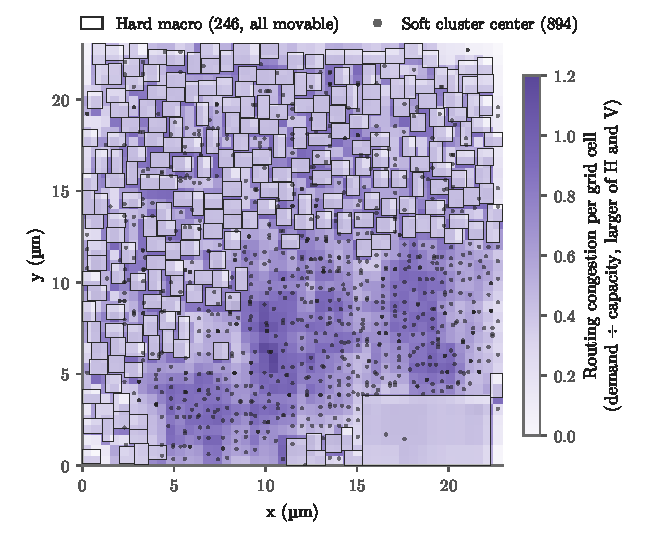
\includegraphics{figures/placement_ibm01.pdf}}%
\begin{minipage}[c]{\wd\sidefigbox}\usebox{\sidefigbox}\end{minipage}\hfill
\begin{minipage}[c]{\dimexpr\linewidth-\wd\sidefigbox-1.2em\relax}
\captionsetup{justification=raggedright,singlelinecheck=false}
\caption{What a placement looks like: IBM01, the smallest design by canvas area and
net count, with 246 hard macros (outlined) and 894 soft-cluster centers on a
$22.95\times23.04\,\mu$m canvas, over the evaluator's routing congestion per grid
cell (darker is more congested). The placement comes from a research run of our
earlier v1 pipeline (\cref{sec:scored}), proxy 0.84528, rescored for this report
(\measurement); the judged entry's coordinates were not saved.}
\label{fig:placement}
\end{minipage}
\end{figure}

The Partcl/HRT Macro Placement Challenge 2026 \citep{challenge2026} posed this
problem on 17 public designs from the ICCAD04 IBM suite
\citep{adya2004unification}, each with 178--786 hard macros and 894--1,985 soft
clusters. Entries were ranked by a \emph{proxy score}, a fast stand-in for the
quality of a fully routed chip: a weighted sum of wirelength, density and routing
congestion computed by an open evaluator \citep{macroplacement} that implements the
Circuit Training proxy \citep{mirhoseini2021graph}.
Lower is better. Any overlap between two hard macros disqualified an entry, and each
design had a one-hour limit.

Two tools pull in opposite directions. A smooth approximation of the score can be
minimized by gradient descent, moving thousands of coordinates together, but it is
only approximate; the exact score is reliable but has kinks and jumps, and judges one
move at a time. Our approach therefore separates proposing moves from accepting them:
a differentiable \emph{surrogate} of the score moves all blocks together, a
\emph{legalizer} moves overlapping hard macros to nearby free spots until none
overlap, and \emph{coordinate descent}, which tries moving one block along one axis
at a time, keeps a move only if the exact score decreases. The ranked configuration
was listed at about 12 minutes per design and placed ninth
(\cref{fig:result-context}). We contribute:
\begin{itemize}[leftmargin=1.6em,topsep=0.3em,itemsep=0.15em]
  \item \textbf{a two-stage placer} in which a smooth surrogate proposes and the
        exact score decides; it is most likely the ranked entry, 31.6\% below the
        published RePlAce baseline and 4.9\% above the winner (\official);
  \item \textbf{exact scoring at local cost}: rescoring only what a move changes
        takes 1.3--3.7\,ms per sampled move against 1.4--26.9\,s for full
        recomputation (\measurement), roughly $10^3$--$2\times10^4$ times faster, so
        a 600\,s search can try about $10^5$ candidate moves instead of at most a
        few hundred; on the sampled states, rounding error is about a million times
        too small to make an accepted move raise the true score;
  \item \textbf{a mathematical framing, from standard tools, that explains the
        design}: for $m$ pairs of blocks the legal region is up to $4^m$ convex
        pieces, which is why one-block moves stay near their starting arrangement
        and the smooth start matters; crowding terms are averages over the worst
        cells, which bounds how far one move can shift them; a Taylor bound says
        when a kick along negative curvature must help a smooth function; and a
        two-block counterexample shows why an optimal reassignment still needs an
        exact recheck;
  \item \textbf{lessons from development records} (\historical): congestion supplied
        84.5\% of our improvement, a pipeline six times faster also scored better,
        and kicks along computed negative-curvature directions helped about equally
        in every direction tried, so the record cannot credit the curvature.
\end{itemize}

\paragraph{How to read this report.} Pages 1--3 and the ``In brief'' boxes tell the
story; \cref{sec:limitations} collects every caveat; the appendices hold the exact
score, settings, proofs, audit, per-design records and a glossary. Each result
carries one evidence label: \official{} for the organizers' final leaderboard,
\historical{} for May 2026 development records (unmatched in hardware, budget and
concurrency, mostly without saved coordinates), and \measurement{} for
post-competition microbenchmarks and diagnostics.
